\documentclass[12pt,a4paper,titlepage,final]{article}

\usepackage[slovak]{babel}
\usepackage[utf8]{inputenc}
% balicky pro odkazy
\usepackage[bookmarksopen,colorlinks,plainpages=false,urlcolor=blue,unicode]{hyperref}
\usepackage{url}
% obrazky
\usepackage{graphicx}
% velikost stranky
\usepackage[top=3.5cm, left=2.5cm, text={17cm, 24cm}, ignorefoot]{geometry}

\usepackage{verbatim}
\begin{document}

%%%%%%%%%%%%%%%%%%%%%%%%%%%%%%%%%%%%%%%%%%%%%%%%%%%%%%%%%%%%%%%%%%%%%%%%%%%%%%
% titulní strana

\def\author{Viktor Jančík}
\def\email{xjanci09@stud.fit.vutbr.cz}
\def\projname{Iteračné výpočty}

\begin{titlepage}

% \vspace*{1cm}
\begin{figure}[!h]
  \centering
  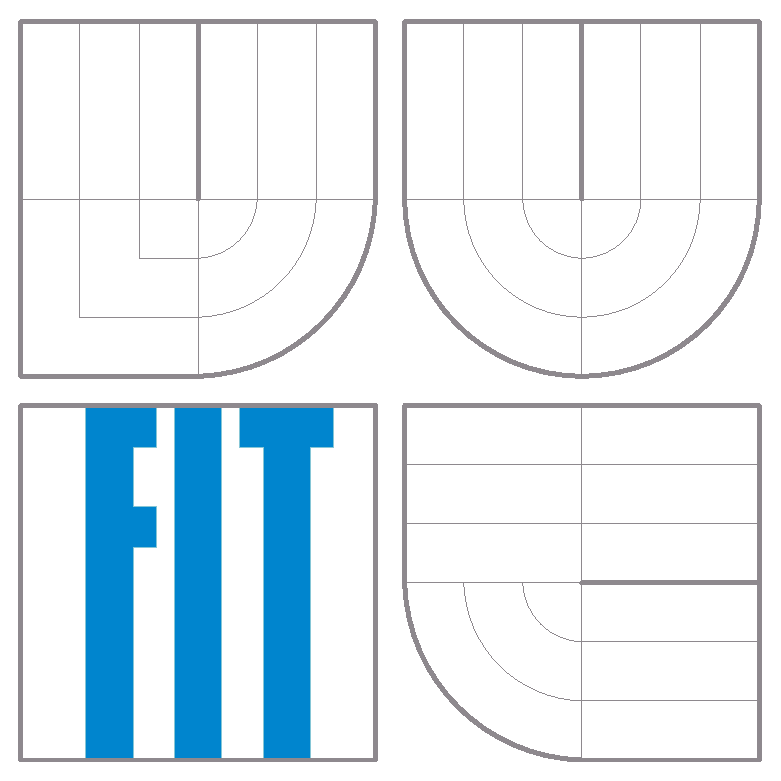
\includegraphics[height=5cm]{img/logo}
\end{figure}

\vfill

\begin{center}
\begin{Large}
Téoria obvodov\\
\end{Large}
\bigskip
\begin{Huge}
Semestrálny projekt\\
\end{Huge}
\end{center}

\vfill

\begin{center}
\begin{Large}
\today
\end{Large}
\end{center}

\vfill

\begin{flushleft}
\begin{large}
\begin{tabular}{ll}
Autor: 
 & Viktor Jančík, \url{xjanci09@stud.fit.vutbr.cz} \\
 & Fakulta Informačních Technologií \\
 & Vysoké Učení Technické v~Brně \\
\end{tabular}
\end{large}
\end{flushleft}
\end{titlepage}


%%%%%%%%%%%%%%%%%%%%%%%%%%%%%%%%%%%%%%%%%%%%%%%%%%%%%%%%%%%%%%%%%%%%%%%%%%%%%%
% obsah
\pagestyle{plain}
\pagenumbering{roman}
\setcounter{page}{1}
\tableofcontents

%%%%%%%%%%%%%%%%%%%%%%%%%%%%%%%%%%%%%%%%%%%%%%%%%%%%%%%%%%%%%%%%%%%%%%%%%%%%%%
% textova zprava
\newpage
\pagestyle{plain}
\pagenumbering{arabic}
\setcounter{page}{1}

%%%%%%%%%%%%%%%%%%%%%%%%%%%%%%%%%%%%%%%%%%%%%%%%%%%%%%%%%%%%%%%%%%%%%%%%%%%%%%
\section{Úvod} \label{uvod}
%%%%%%%%%%%%%%%%%%%%%%%%%%%%%%%%%%%%%%%%%%%%%%%%%%%%%%%%%%%%%%%%%%%%%%%%%%%%%%
Iteračné výpočty sú výpočty hodnôt pomocou iterácie, a teda opakovania nejakého výpočtu. S každou iteráciou sa výsledok tohto výpočtu čoraz viac približuje k presnému očakávanému výsledku výpočtu. V~počítačoch je však málokedy niečo úplne presné, najmä keď pracujeme s číslami s desatinným rozvojom. Vždy hovoríme o akejsi úrovni presnosti, teda počet desatinných miest, v ktorom sa výpočet zhoduje s presnou hodnotou výsledku.

Tento dokument sa zaoberá návrhom a implementáciou programu pre výpočet funkcie tangens a výpočet veľkosti a vzdialenosti meraného objektu na základe uhla, ktorý zviera s meracím prístrojom. Funkciu tangens program počíta iteračnými výpočtami s určitým počtom iterácií. Výsledný program je konzolová aplikácia, ktorá príma textový vstup zo štandardného vstupu, vykonáva tieto výpočty a vypisuje výsledok týchto výpočtov na štandardný výstup.

Dokument má viacero častí. Kapitola \ref{analyza} sa zaoberá analýzou problému a možnými spôsobmi riešenia. Kapitola \ref{navrh} sa zaoberá konkrétnym návrhom riešenia a v kapitole \ref{riesenie} je popísaná implementácia riešenia tohto problému. V kapitole  \ref{testy} je niekoľko testovacích vstupov a výstupov, ktoré boli použité pre kontrolu správnosti programu.

%%%%%%%%%%%%%%%%%%%%%%%%%%%%%%%%%%%%%%%%%%%%%%%%%%%%%%%%%%%%%%%%%%%%%%%%%%%%%%
\section{Analýza problému a princíp jeho riešenia} \label{analyza}
%%%%%%%%%%%%%%%%%%%%%%%%%%%%%%%%%%%%%%%%%%%%%%%%%%%%%%%%%%%%%%%%%%%%%%%%%%%%%%

V tejto kapitole sa budem hlbšie venovať problematike počítania s číslami s desatinným rozvojom reprezentovanými v počítači ako čísla s pohyblivou desatinnou čiarkou. Ďalej sa budem zaoberať počítaním funkcie tangens vrámci limitácií počítačov, spôsobmi počítania funkcie tangens a zadaním projektu.

%=============================================================================
\subsection{Zadanie problému}

Úlohou projektu vytvoriť konzolovú aplikáciu v jazyku C, ktorá dokáže vypočítať vzdialenosť a výšku meraného objektu pomocou údajov zo senzoru, v podobe uhlov $\alpha$, $\beta$ a výšky meraného prístroja. Situácia je ilustrovaná obrázkom \ref{fig:obrazok1}.
 
Uhol $\alpha$ reprezentuje uhol, ktorý zviera merací prístroj s meraným objektom od úrovne výšky meracieho prístroja po spodnú hranicu objektu. Uhol $\beta$ reprezentuje uhol, ktorý zviera merací prístroj s meraným objektom od úrovne výšky meracieho prístroja po hornú hranicu objektu. Dĺžka \textit{c} značí výšku meracieho prístroja od pomyslenej zeme. Dĺžka \textit{v} značí výšku meraného objektu a dĺžka \textit{d} značí vzdialenosť objektu od meracieho prístroja.

Pre výpočet vzdialenosti a výšky meraného objektu budeme potrebovať výpočet funkcie tangens uhlov $\alpha$ a $\beta$. 


Ďalšia požiadavka pre program, je samostatný výpočet funkcie tangens na špecifikovaný počet iterácií, troma spôsobmi, a to funkciou \texttt{double tan(double x);} z knižnice \texttt{math.h}, Taylorovým polynómom a metódou zreťazených zlomkov. V tomto prípade je výstupom programu výsledná hodnota tangens pre každú iteráciu v určenom rozsahu iterácií, pre každú z týchto troch metód\footnote{Výsledok funkcie \textit{tan} z knižnice \texttt{math.h} nie je ovplyvnený počtom iterácií a slúži ako referenčná hodnota.}. Súčasťou výstupu je zároveň porovnanie presnosti každej z týchto metód pre danú iteráciu, voči presnej hodnote.

%=============================================================================
\subsection{Špecifiká zadania problému}\label{specifikacia}

Zadanie špecifikuje nutnosť výpočtu funkcie tangens pre výpočet výšky a vzdialenosti meraného objektu metódou zreťazených zlomkov s presnosťou aspoň na desať cifier za desatinnou čiarkou.

Pre uhol $\alpha$, $\beta$ a výšku \textit{c}, zadanie udáva rozsah hodnôt, pre ktoré musí mať program správny výstup:
\begin{equation}\label{eq:limAlpha} 
0 < \alpha \leq 1.4 < \frac{\pi}{2}
\end{equation}
\begin{equation}\label{eq:limBeta} 
0 < \beta \leq 1.4 < \frac{\pi}{2}
\end{equation}
\begin{equation}\label{eq:limC} 
0 < c \leq 100
\end{equation}

Pre výpočet Taylorového polynómu a zreťazeného zlomku, zadanie vyžaduje implementovanie funkcií s týmito prototypmi:

\begin{verbatim}
double taylor_tan(double x, unsigned int n);
double cfrac_tan(double x, unsigned int n);
\end{verbatim}

Pre počet iterácií \textit{I} výpočtu platí:
\begin{equation}
0 < I < 14
\end{equation}


%=============================================================================
\subsection{Presnosť a počítanie s číslami s pohyblivou desatinnou čiarkou} \label{presnost}

\begin{figure}
  \centering
  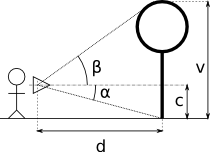
\includegraphics[scale=1]{img/Diagram.png}
  \caption{Ilustračný obrázok popisujúci vzťahy medzi meracím prístrojom a meraným objektom.}
  \label{fig:obrazok1}
\end{figure}

V počítačoch sú všetky dáta uložené ako reťazce bitov (núl a jednotiek). Konečným počtom bitov sa dá reprezentovať konečný počet unikátnych hodnôt. Napríklad dátový typ  \texttt{double}, ktorý používa 64 bitov pamäte, dokáže reprezentovať 15 až 17 platných decimálnych číslic\footnote{\label{FNPresnost}Presný počet závisí od štandardu, podľa ktorého sa riadi implementácia v danom programovaciom jazyku.}.

Z toho vyplýva, že pre akékoľvek iteračné výpočty s týmto dátovým typom sa oplatí počítať len do presnosti (maximálne) \textit{$10^{-17}$}. Po dosiahnutí tejto presnosti, ďalšie iterácie nemajú vplyv na výsledok výpočtu, pretože cifry, ktoré sa menia niesu zobraziteľné v 64 bitoch pamäte.

Na porovnanie, dátový typ \texttt{float}, ktorý používa 32 bitov pamäte, dokáže reprezentovať 6 až 9 platných decimálnych číslic\textsuperscript{\ref{FNPresnost}}.

%=============================================================================
\subsection{Taylorov polynóm}

Taylorov polynóm je spôsob reprezentácie funkcie ako nekonečnú sumu členov, vypočítaných z hodnôt derivácií (rôznych stupňov) funkcie pre konkrétnu hodnotu.
Všeobecný tvar Taylorového polynómu je:
\begin{equation}\label{eq:taylor1} 
\sum\limits_{n=0}^\infty \frac{f^{(n)}(a)}{n!}(x-a)^n
\end{equation}

Kde $f^{(n)}(a)$ reprezentuje n-tú deriváciu funkcie \textit{f} v bode \textit{a}.

Špecifický tvar Taylorového polynómu pre funkciu \textit{tan(x)} je:
\begin{equation}\label{eq:taylor2} 
tan(x) = x + \frac{x^3}{3} + \frac{2x^5}{15} + \frac{17x^7}{315} + \frac{62x^9}{2935} +...
\end{equation}

V kontexte tohto projektu uvažujeme pripočítanie ďalšieho člena postupnosti k výsledku ako jednu iteráciu výpočtu.

%=============================================================================
\subsection{Zreťazené zlomky}

Metóda zreťazených zlomkov je metóda výpočtu funkcie pomocou nekonečného reťazca zlomkov. Pre výpočet funkcie \textit{tan(x)} má zreťazený zlomok tvar \ref{eq:cfrac1} alebo \ref{eq:cfrac2}:

\begin{equation}\label{eq:cfrac1} 
tan(x) = \frac{x}{1 - \frac{x^2}{3 - \frac{x^2}{5 - \frac{x^2}{7 -...}}}}
\end{equation}

\begin{equation}\label{eq:cfrac2} 
tan(x) = \frac{1}{\frac{1}{x} - \frac{1}{\frac{3}{x} - \frac{1}{\frac{5}{x} - \frac{1}{\frac{7}{x} -...}}}}
\end{equation}

V kontexte tohto projektu uvažujeme pridanie ďalšej úrovne zlomku ako jednu iteráciu výpočtu.

%=============================================================================
\subsection{Princíp riešenia výpočtu výšky a vzdialenosti meraného objektu}

Je viacero možností ako vypočítať výšku a vzdialenosť meraného objektu. Zadanie projektu si vyžaduje pre tento výpočet použitie funkcie pre výpočet tangens pomocou zreťazených zlomkov. Vzhľadom na tento fakt a vstupné hodnoty (uhol $\alpha$, $\beta$; výška \textit{c}) je intuitívne vypočítať výšku a vzdialenosť objektu pomocou trigonometrických vzťahov, na trojuholníkoch, ktoré zadané uhly a veľkosti špecifikujú.

%%%%%%%%%%%%%%%%%%%%%%%%%%%%%%%%%%%%%%%%%%%%%%%%%%%%%%%%%%%%%%%%%%%%%%%%%%%%%%
\section{Návrh riešenia problému} \label{navrh}
%%%%%%%%%%%%%%%%%%%%%%%%%%%%%%%%%%%%%%%%%%%%%%%%%%%%%%%%%%%%%%%%%%%%%%%%%%%%%%

Požiadavkami v zadaní problému je riešenie takmer presne definované. Presnejšie, aby sme splnili tieto požiadavky, dá sa použiť akurát jedno riešenie. V tejto kapitole opíšem spôsob implementácie výpočtov potrebných pre podproblémy môjho programu, zatiaľ čo v kapitole \ref{riesenie} sa budem venovať implementačným detailom.

%=============================================================================
\subsection{Výpočet Taylorového polynómu}\label{impTaylor}

Taylorov polynóm pre funkciu tangens som vypočítal podľa vzorca \ref{eq:taylor2}. Pre tento vzorec však potrebujem vypočítať hodnoty koeficientov pre každý člen postupnosti. Vzorec pre výpočet týchto koeficientov je netriviálny, preto, keďže poznám maximálny počet iterácií, ktoré budú požadované, je efektívnejšie uložiť hodnoty týchto koeficientov pre prvých 13 iterácií do poľa. 

Sú to tieto koeficienty v čitateli\cite{taylorNum}:
\begin{verbatim}
1, 1, 2, 17, 62, 1382, 21844, 929569, 6404582, 443861162, 18888466084,
113927491862, 58870668456604, 8374643517010684, 689005380505609448,
129848163681107301953, 1736640792209901647222, 418781231495293038913922
\end{verbatim}

A tieto hodnoty pre koeficienty v menovateli\cite{taylorDenom}:
\begin{verbatim}
1, 3, 15, 315, 2835, 155925, 6081075, 638512875, 10854718875, 1856156927625,
194896477400625, 49308808782358125, 3698160658676859375,
1298054391195577640625, 263505041412702261046875
\end{verbatim}

%=============================================================================
\subsection{Výpočet zreťazeného zlomku} \label{cfracNavrh}

Výpočet zreťazeného zlomku je trochu zložitejší (aspoň na pohľad), pretože narozdiel od Taylorového rozvoju kde jasne akumulujeme členy postupnosti, pri zreťazenom zlomku, nie je na prvý pohľad jasné, čo vlastne máme akumulovať.

Pri zreťazenom zlomku akumulujeme menovateľ zlomku odspodu, pričom uvažujeme, že tento menovateľ v nekonečne naberá hodnotu 0.

Pre výpočet som si zvolil vzorec \ref{eq:cfrac1}. Po akumulácií zlomku na niekoľko úrovní (dané počtom iterácií), predelím čitateľ týmto menovateľom a dostanem správnu hodnotu.

\subsection{Výpočet vzdialenosti a výšky objektu}\label{measures}

Z trigonometrie sa dajú ľahko odvodiť nasledujúce vzorce pre výpočet vzdialenosti a výšky objektu (symboly podľa obrázku \ref{fig:obrazok1}):

\begin{equation}
d = \frac{c}{tan(\alpha)}
\end{equation}

\begin{equation}
v = tan(\beta)*d + c
\end{equation}

Presnosť výpočtu funkcie tangens na desať cifier po desatinnej čiarke zaručujem opakovaným počítaním funkcie tangens, až kým rozdiel výsledkov dvoch po sebe idúcich iterácií výpočtu nie je menší ako $10^{-10}$.

%=============================================================================
%=============================================================================
\section{Špecifikácia testov} \label{testy}

Na základe hraníc vstupných hodnôt a návrhu riešenia vznikajú krajné situácie, pre ktoré treba otestovať správnosť algoritmu.

\paragraph{Test 1:} Prvý vzorový príklad vstupu a výstupu zo zadania projektu.

\vspace{1em}\begin{tabular}{l}
vstup \\
\hline
\verb|./proj2 --tan 1.024 6 10|
\end{tabular}

\vspace{1em}\begin{tabular}{l}
očakávaný výstup \\
\hline
\verb|6 1.642829e+00 1.634327e+00 8.502803e-03 1.642829e+00 3.298801e-09| \\
\verb|7 1.642829e+00 1.639216e+00 3.613451e-03 1.642829e+00 1.794520e-11| \\
\verb|8 1.642829e+00 1.641294e+00 1.535615e-03 1.642829e+00 7.460699e-14| \\
\verb|9 1.642829e+00 1.642177e+00 6.525932e-04 1.642829e+00 4.440892e-16| \\
\verb|10 1.642829e+00 1.642552e+00 2.773337e-04 1.642829e+00 0.000000e+00| 
\end{tabular}

\paragraph{Test 2:} Druhý vzorový príklad vstupu a výstupu zo zadania projektu.

\vspace{1em}\begin{tabular}{l}
vstup \\
\hline
\verb|./proj2 -m 0.3 0.9|
\end{tabular}

\vspace{1em}\begin{tabular}{l}
očakávaný výstup \\
\hline
\verb|4.8490922156e+00| \\
\verb|7.6106234032e+00|
\end{tabular}

\paragraph{Test 3:} Tretí vzorový príklad vstupu a výstupu zo zadania projektu.

\vspace{1em}\begin{tabular}{l}
vstup \\
\hline
\verb|./proj2 -c 1.7 -m 0.15 1.3|
\end{tabular}

\vspace{1em}\begin{tabular}{l}
očakávaný výstup \\
\hline
\verb|1.1248205560e+01| \\
\verb|4.2217188781e+01|
\end{tabular}

\paragraph{Test 4:} Tangens uhla 0.

\vspace{1em}\begin{tabular}{l}
vstup \\
\hline
\verb|./proj2 --tan 0 1 3|
\end{tabular}

\vspace{1em}\begin{tabular}{l}
očakávaný výstup \\
\hline
\verb|1 0.000000e+00 0.000000e+00 0.000000e+00 0.000000e+00 0.000000e+00| \\
\verb|2 0.000000e+00 0.000000e+00 0.000000e+00 0.000000e+00 0.000000e+00| \\
\verb|3 0.000000e+00 0.000000e+00 0.000000e+00 0.000000e+00 0.000000e+00|
\end{tabular}

\paragraph{Test 5:} Tangens uhla väčšieho ako $\frac{\pi}{2}$ (využitie periódy funkcie tangens).

\vspace{1em}\begin{tabular}{l}
vstup \\
\hline
\verb|./proj2 --tan 2 11 13|
\end{tabular}

\vspace{1em}\begin{tabular}{l}
očakávaný výstup \\
\hline
\verb|11 4.576576e-01 2.132589e+00 -1.674932e+00 4.576576e-01 0.000000e+00| \\
\verb|12 4.576576e-01 2.132589e+00 -1.674932e+00 4.576576e-01 0.000000e+00| \\
\verb|13 4.576576e-01 2.132589e+00 -1.674932e+00 4.576576e-01 0.000000e+00|
\end{tabular}

\paragraph{Test 6:} Tangens záporného uhla (kontrola symetrie).

\vspace{1em}\begin{tabular}{l}
vstup \\
\hline
\verb|./proj2 --tan -1.024 8 10|
\end{tabular}

\vspace{1em}\begin{tabular}{l}
očakávaný výstup \\
\hline
\verb|8 -1.642829e+00 -1.641294e+00 -1.535615e-03 -1.642829e+00 -7.460699e-14| \\
\verb|9 -1.642829e+00 -1.642177e+00 -6.525932e-04 -1.642829e+00 -4.440892e-16| \\
\verb|10 -1.642829e+00 -1.642552e+00 -2.773337e-04 -1.642829e+00 0.000000e+00| 
\end{tabular}


%%%%%%%%%%%%%%%%%%%%%%%%%%%%%%%%%%%%%%%%%%%%%%%%%%%%%%%%%%%%%%%%%%%%%%%%%%%%%%
\section{Popis riešenia} \label{riesenie}
%%%%%%%%%%%%%%%%%%%%%%%%%%%%%%%%%%%%%%%%%%%%%%%%%%%%%%%%%%%%%%%%%%%%%%%%%%%%%%

Implementácia programu vychádza zo záverov predošlých kapitol. V tejto kapitole sa budem zaoberať detailami implementácie v jazyku C.

%=============================================================================
\subsection{Ovládanie programu}

Program je implementovaný ako konzolová aplikácia. Spustiť ju je možne s rôznymi vstupnými parametrami\footnote{Presný popis vstupných parametrov je rozsiahly a vypíše sa v prípade spustenia programu s parametrom \texttt{--help}.}:

\begin{verbatim}
./proj2 --help
./proj2 --tan A N M
./proj2 [-c X] -m A [B]
\end{verbatim}

V prípade, že sa vstupné parametre nebudú zhodovať ani s jedným z týchto vzorov, program sa ukončí, bez akéhokoľvek výstupu. Ak sa nedodrží rozsah hodnôt špecifikovaný v zadaní projektu, správanie programu nie je definované.

Pre výpočet funkcie tangens (volanie s parametrom \texttt{--tan}) má výstup formát:

\begin{verbatim}
I M T TE C CE
\end{verbatim}

Vypísaný formátom \texttt{"\%d \%e \%e \%e \%e \%e$\backslash$n"}, funkciou \texttt{printf}, kde:
\begin{itemize}
\setlength\itemsep{0em}
\item I značí počet iterácií iteračného výpočtu, 
\item M výsledok z funkcie tan matematickej knižnice,
\item T výsledok z funkcie taylor\_tan,
\item TE absolútnu chybu medzi výpočtom pomocou Taylorového polynómu a matematickou knižnicou,
\item C výsledok z funkcie cfrac\_tan a
\item CE absolútnu chybu medzi výpočtom pomocou zreťazených zlomkov a matematickou knižnicou.
\end{itemize}

Pre výpočet vzdialenosti a výšky (volanie s parametrom \texttt{--m}) ma výstup formát\footnote{Obidve hodnoty sú vypísané formátom \texttt{\%.10e}}:

\begin{verbatim}
vzdialenosť výška
\end{verbatim}

%=============================================================================
\subsection{Voľba dátových typov}

Pre hodnoty výpočtov funkcie tangens (všetky metódy) som použil dátový typ \texttt{double}, pretože by dátový typ \texttt{float} nedokázal zobraziť požadovanú presnosť hodnôt (sekcia \ref{specifikacia}), z dôvodov opísaných v sekcii \ref{presnost}.

%=============================================================================
\subsection{Špecifikácia výpočtu zreťazeného zlomku}

V predchádzajúcej kapitole (sekcia \ref{cfracNavrh}) som načrtol problematiku akumulovania menovateľa pre výpo\-čet zreťazeného zlomku. Presná implementácia tohto procesu je:

\begin{verbatim}
for(int i=(n+1); i>0; --i) {
    denominator = (2*i - 1) - xx/denominator;
}
\end{verbatim}

Kde \texttt{n} je počet iterácií, \texttt{xx} je $uhol^2$ a \texttt{denominator} je menovateľ zreťazeného zlomku.

Počiatočná hodnota \texttt{denominator} je 0 (menovateľ v nekonečne).

%=============================================================================
\subsection{Vlastná implementácia}

Parametre zo štandardného vstupu sú spracovávané vo funkcii \texttt{main}. Na základe tohto spracovania sa spustí buď funkcia \texttt{comp\_tan}, ktorá je zodpovedná, za spúšťanie \texttt{taylor\_tan}, \texttt{cfrac\_tan} a správne vypisovanie a formátovanie výstupu pre výpočet funkcie tangens, alebo sa spustí funkcia \texttt{measures}, ktorá pomocou funkcie \texttt{cfrac\_tan} a vzťahov zo sekcie \ref{measures} vypočíta a vypíše vzdialenosť a výšku meraného objektu, tiež v správnom formáte. V prípade spustenia programu so vstupným argumentom \texttt{--help}, sa spustí funkcia \texttt{print\_desc} a vypíše popis funkcií programu.

Program taktiež zahŕňa pomocnú funkciu \texttt{power} ktorá vráti n-tú mocninu daného čísla (používa sa pre \texttt{taylor\_tan}).

Koeficienty pre výpočet Taylorového polynómu funkcie tangens sú uložené v poliach 
\\*\texttt{taylorNum} a \texttt{taylorDenom}.

%=============================================================================
\subsection{Optimalizačné detaily}

Pre optimalizáciu výpočtu som použil globálnu štruktúru \texttt{partialResult}, ktorá obsahuje číslo iterácie výpočtu (alebo stupeň mocniny - v prípade \texttt{prPower}) a čiastočný výsledok. Konkrétne, \texttt{prTaylor}, sa používa na optimalizáciu výpočtu Taylorového polynómu. Samozrejme by globálna premenná nemusela byť použitá v prípade, že by funkcia \texttt{taylor\_tan} nemala vopred stanovený prototyp, ktorý som musel dodržať.

V prípade výpočtu zreťazeného zlomku, sa týmto spôsobom výpočet optimalizovať nedal, pretože čiastočné výpočty, a teda čiastočná akumulácia menovateľa zlomku, nemá pre konkrétny počet iterácií význam.

Funkcia \texttt{power} je z dôvodu jednoduchosti použiteľná len pre jednu hodnotu počas celého behu programu. To však správnosti tohto programu neprekáža.

%%%%%%%%%%%%%%%%%%%%%%%%%%%%%%%%%%%%%%%%%%%%%%%%%%%%%%%%%%%%%%%%%%%%%%%%%%%%%%
\section{Záver} \label{zaver}
%%%%%%%%%%%%%%%%%%%%%%%%%%%%%%%%%%%%%%%%%%%%%%%%%%%%%%%%%%%%%%%%%%%%%%%%%%%%%%

Program spĺňa všetky požiadavky zo zadania problému. Navyše program optimalizuje opakovaný výpočet Taylorového polynómu alebo mocniny konkrétneho čísla. Program by sa dal ešte vylepšiť sprísnením kontroly vstupných argumentov z príkazového riadku, ale pre korektný (podľa špecifikácie zadania problému) vstup, program vždy vráti korektný výstup. 

Program bol vyvíjaný a testovaný na operačnom systéme Ubuntu (Linux), ale mal by fungovať pre všetky platformy, ktoré podporujú jazyk C a štandard C99, keďže program nepoužíva žiadne systémovo závisle funkcionality.

%%%%%%%%%%%%%%%%%%%%%%%%%%%%%%%%%%%%%%%%%%%%%%%%%%%%%%%%%%%%%%%%%%%%%%%%%%%%%%
% seznam citované literatury: každá položka je definována příkazem
% \bibitem{xyz}, kde xyz je identifikátor citace (v textu použij: \cite{xyz})
\begin{thebibliography}{2}

\bibitem{taylorNum}
A002430 - OEIS. [online]. [cit. 2014-12-05]. Dostupné z: https://oeis.org/A002430

\bibitem{taylorDenom}
A156769 - OEIS. [online]. [cit. 2014-12-05]. Dostupné z: https://oeis.org/A156769

\end{thebibliography}
%%%%%%%%%%%%%%%%%%%%%%%%%%%%%%%%%%%%%%%%%%%%%%%%%%%%%%%%%%%%%%%%%%%%%%%%%%%%%%
% přílohy
\appendix

\section{Metriky kódu} \label{metriky}
\paragraph{Počet súborov:} 1 súbor
\paragraph{Počet riadkov zdrojového kódu:} 137 riadkov
\paragraph{Veľkosť statických dat:} 936B
\paragraph{Veľkosť spustiteľného súboru:} 5396B (systém Linux, 32 bitová
architektúra, pri preklade bez ladiacich informácii)

\end{document}
